\graphicspath{{./images/}}
% Configure style


\titleformat{\section}
{\normalfont\fontfamily{phv}\fontsize{10}{0}\bfseries}{\thesection}{1em}{}
\section{Using Transformers}
\renewcommand\labelitemi{{\boldmath$\cdot$}}
\setlist{nolistsep}
\begin{itemize}[noitemsep]
    \item How does Pipeline work?
    \item 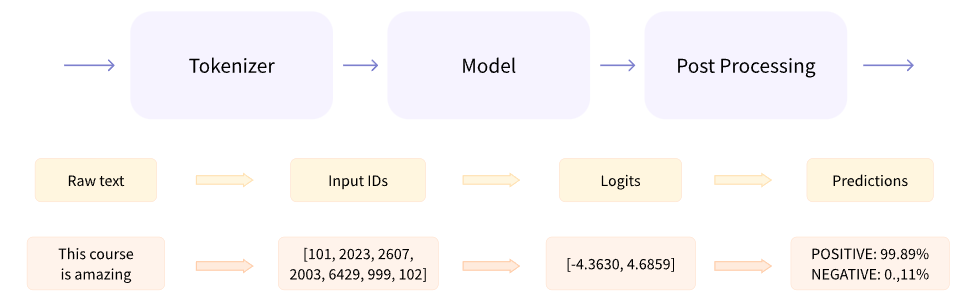
\includegraphics[height=0.3\linewidth]{pipeline_architecture.png}
    \begin{lstlisting}
                    import torch
                    from transformers import AutoTokenizer, AutoModelForSequenceClassification

                    checkpoint = "distilbert-base-uncased-finetuned-sst-2-english"
                    tokenizer = AutoTokenizer.from_pretrained(checkpoint)
                    model = AutoModelForSequenceClassification.from_pretrained(checkpoint)
                    sequences = ["I've been waiting for a HuggingFace course my whole life.", "So have I!"]

                    tokens = tokenizer(sequences, padding=True, truncation=True, return_tensors="pt")
                    output = model(**tokens)
    \end{lstlisting}
    \item Tokenizers
    \begin{itemize}[noitemsep]
        \item Word-based - splits by spaces but often generates too many [UNK] tokens
        \item Character-based - splits into characters but generates too many tokens
        \item Subword-based - balances vocabulary size and coverage. 
        For example, "tokenization" would be split into "token", "ization" 
    \end{itemize}
\end{itemize}